\subsection{Arquitectura de conversión de datos}

La arquitectura del Modelo de Información de Integración de openEHR, mostrado en la Figura \ref{fig:data_conversion_architecture}, está diseñado para situaciones de integración heredadas.

\begin{figure}[h]
  \centering
  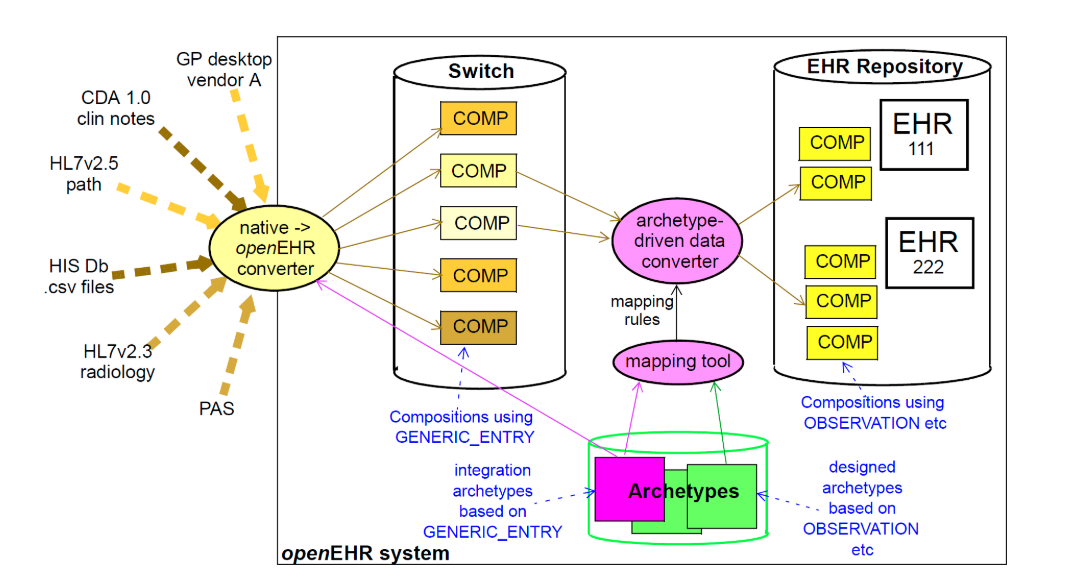
\includegraphics[scale=0.4]{./images/data_conversion_architecture}
  \caption{Integración de dato dentro de openEHR (Fuente: Extraído desde \cite{openEHR}).}
  \label{fig:data_conversion_architecture}
\end{figure}

La base del diseño se basa en una clara separación de la transformación sintáctica y semántica requerida en los datos importados en openEHR. La transformación sintáctica convierte los datos de su formato sintáctico original en estructuras del modelo de referencia de openEHR, cuya estructura lógica y semántica está controladas por arquetipos de integración que imitan el diseño original de los datos. Como resultado de la conversión, los datos son susceptibles de ser procesados en openEHR. La transformación semántica convierte los datos importados a arquetipos clínicos.

Los elementos de openEHR que hacen posible esta transformación son:
\begin{itemize}
  \item la clase GENERIC\_ENTRY que se utiliza para crear representaciones intermedias de datos de fuentes que de otra manera no se ajustan a las clases openEHR;
  \item arquetipos de integración definidos en contra de la clase GENERIC\_ENTRY;
  \item reglas de transformación semántica de los datos de openEHR basados en GENERIC\_ENTRY y arquetipos de integración a los datos basados en los subtipos de ENTRY, y arquetipos clínicos diseñados.
\end{itemize}
